
\chapter{Desarrollo}
\label{chap:desarrollo}
\vspace{0.5cm}

\lettrine{E}{n} este capítulo se desarrollarán los detalles de la implementación de los diferentes módulos de interacción que se han diseñado para el ROBOBO así como la metodología de trabajo seguida.
%%%%%%%%%%%%%%%%%%%%%%%%%%%%%%%%%%%%%%%%%%%%%%%%%%%%%%%%%%%%%%%%%%%%%%%%%%%%%%%%
% Objetivo: Exponer las partes relevantes de la implementación                 %
%%%%%%%%%%%%%%%%%%%%%%%%%%%%%%%%%%%%%%%%%%%%%%%%%%%%%%%%%%%%%%%%%%%%%%%%%%%%%%%%
%TODO Introducción al capitulo
\section{Capacidades de interacción del ROBOBO}
\label{sec:capacidades-interactivas}

El ROBOBO gracias a la combinación de Smartphone (OBO) y base motorizada (ROB) presenta un gran potencial de formas de interacción.

El OBO, pone a nuestra disposición todas las características de un teléfono inteligente moderno que, diseñado específicamente para su uso por humanos, ofrece múltiples posibilidades y capacidades que facilitan el desarrollo de un sistema de interacción.
\begin{itemize}
	\item \textbf{Gran capacidad de procesado de datos}, que nos permite procesar, por ejemplo, las imágenes capturadas por la cámara para desarrollar métodos de interacción complejos, como detección de caras o colores
	\item Variedad de sensores:
	\begin{itemize}
		\item \textbf{Acelerómetro, giroscopio y magnetómetro}, permiten al robot tener conciencia de su posición espacial
		\item \textbf{Sensores de luz ambiente}, que permiten reaccionar a los cambios lumínicos del entorno
		\item \textbf{Micrófono}, que permite escuchar su entorno y actuar en consecuencia
		\item \textbf{Cámara frontal y trasera}, que permiten capturar imágenes y procesarlas posteriomente
	\end{itemize}
	\item \textbf{Pantalla táctil de alta resolución}, que permite interacción en dos direcciones, ya sea mediante gestos táctiles como mediante gráficos en la pantalla
	\item \textbf{Conexión a internet}, que permite al robot comunicarse a través de este medio.
	\item \textbf{Altavoces}, permiten interacción mediante sonidos, música y habla.
\end{itemize}

\begin{figure}[h]
	\centering
	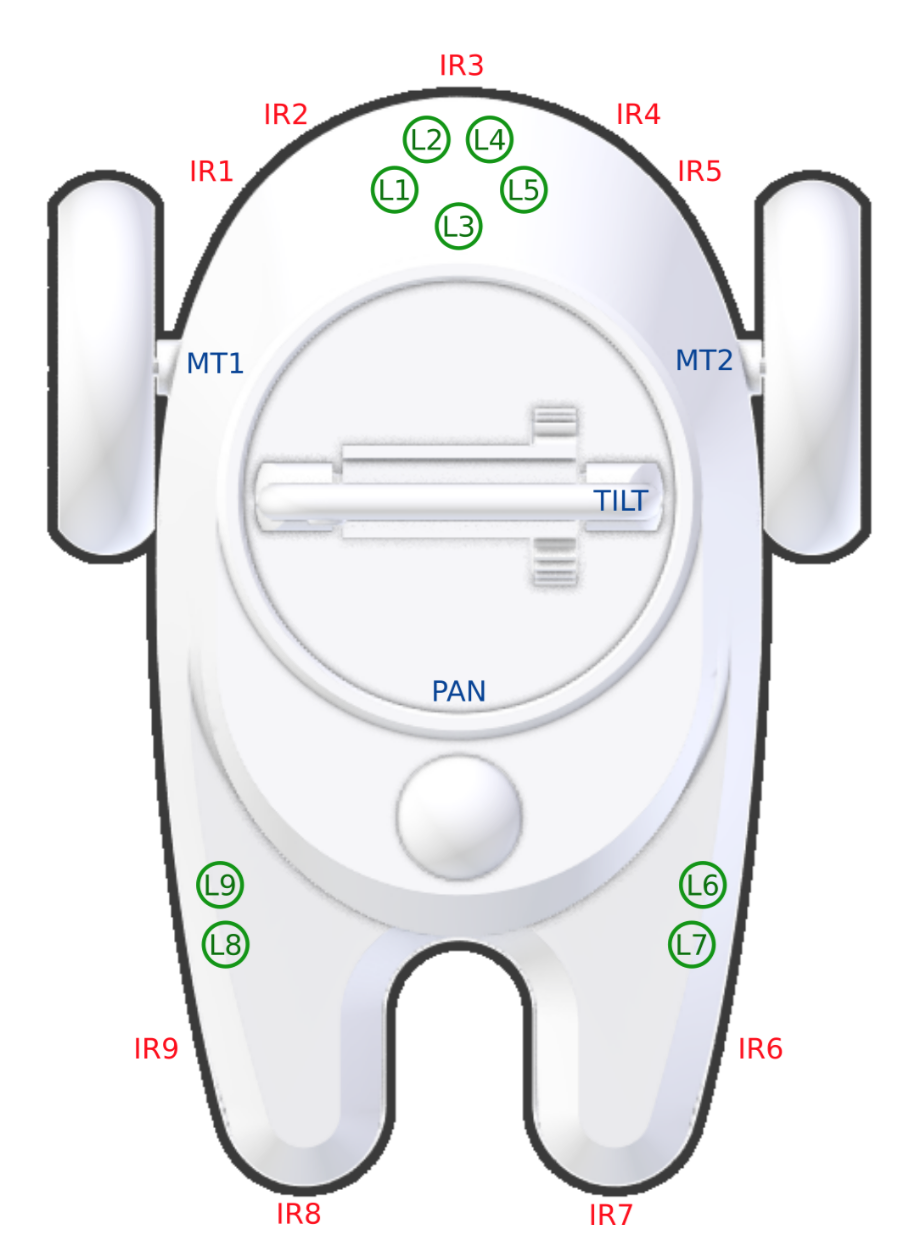
\includegraphics[width=0.4\linewidth]{imagenes/rob_schema.png}
	\caption{Esquema de sensores y actuadores del ROB}
	\label{fig:rob-schema}
\end{figure}
El ROB, cuyo esquema de sensores y actuadores podemos ver en la figura \ref{fig:rob-schema}, proporciona ciertas posibilidades de interacción ya sea mediante sus motores, por ejemplo a través de bailes y gestos, como utilizando los 9 leds RGB que se encuentran a lo largo del chasis para expresar diferentes cosas.

Combinando ambas partes se obtiene un robot con un gran potencial para establecer interacción con personas.



%Gervasio: Las secciones 5.1 y 5.2 las veo bastante bien, pero me falta un analisis del Robobo en terminas de sus capadiaddes de interacción. Es decir, en la 5.1 entras ya muy a saco, ya vas al granto, queremos esto, estoy y esto.
%Creo que quedaría bien añadir una sección anterior en la que presentas al ROBOBO (como en la 2) pero en términos de sus capacidades de interacción. Por ejemplo (pero con más chicha):
%- En el OBO, gracias a que es un Smartphone, tenemos una gran variedad de hardware pensado para interactuar con personas, por ejemplo la pantalla táctil que tal y cual, altavoces para XXX, cámara… además tenemos una gran capacida de preocsamiento, etc.
%- En el ROB tenemos difrentes capacidades de movimiento para interactuar con “gestos” del robot, bailes, etc., LEDs para indicar cosas, etc.
%A partir de ahí vas a la 5.1, donde dices, “Ok, con todo lo anterior vamos a hacer un sistema de interacción con estos ‘sentidos’, siguiendo los ejemplos”.

\section{Modelo conceptual para el subsistema de interacción}
 \label{sec:modelo-conceptual}
 
 %La plataforma ROBOBO, cuenta con características que permiten realizar diversas maneras de interacción, el hecho de estar basado en un smartphone, pone todas las capacidades del mismo a disposición a la hora de interactuar con los usuarios. 
 
 Partiendo de las características expuestas en el punto anterior y basándose en los ejemplos de interacción mostrados en el capítulo anterior se han definido, en una analogía a los sentidos, una serie de paquetes para dotar al ROBOBO de diversas funcionalidades de interacción.
 
 El primero de estos paquetes sería el \enquote{sentido} de habla, que en la sección anterior se pudo ver su aplicación en robots como Nao, Dash y Dot. Siendo el habla, probablemente, la principal forma de interacción que se da entre los humanos, parece lógico que, teniendo la capacidad de proceso de un smartphone moderno, dotar al robot ya no solo de la capacidad de producir habla, sino de entender texto hablado es un concepto interesante. Este paquete daría al robot la posibilidad de comunicación bidireccional con los humanos, además de darle al robot cierta personalidad más \enquote{orgánica} , haciéndolo más atractivo, por ejemplo, a los niños.
 
 El segundo, de forma análoga al sentido del tacto, teniendo una \enquote{piel artificial} cómo es la pantalla táctil del teléfono, dar la capacidad al robot de sentir toques y caricias parece una idea interesante a la hora de llevar una interacción cercana con el robot, este tipo de interacción mediante toques en la pantalla táctil es similar al del SmartPet, y de una manera más general, al sentido del tacto del robot Paro o el Aibo.
 
 El tercero, siguiendo la analogía con los sentidos, sería el sentido del oído. La capacidad de producir y reconocer sonidos abre puertas a tipos de interacción interesantes. Por ejemplo, la capacidad de reaccionar ante sonidos fuertes como palmadas o la capacidad de reconocer notas musicales podrían permitir al robot comunicarse mediante el uso de la música, y estando el ROBOBO enfocado directamente a la educación, esta clase de interacción podría emplearse para la enseñanza musical en la educación infantil y primaria. También, la producción de sonidos, es una forma de comunicación que parece adecuada a la hora de interactuar con niños, ya sea mediante sonidos básicos (risas, alarmas, abucheos...)  como a través de notas musicales, que podría usarse en conjunto con la capacidad de reconocimiento de las mismas a la hora de la enseñanza musical. Esta capacidad de producir música se puede ver en el robot Dash mediante el módulo del xilófono y la de detección de música y palmadas en el Zowi.
 
 El cuarto paquete, teniendo hoy en día todos los smartphones como mínimo una cámara, busca dotar al ROBOBO de sentido de la vista. Con este sentido, el robot podría detectar la presencia de gente y a que distancia se encuentran y de esta manera adaptar su comportamiento a su entorno, por ejemplo, alejándose si nota que alguien esta muy cerca o siguiendo con la \enquote{cara} a la gente a su alrededor. La capacidad de discernir diferentes colores también es una habilidad interesante de cara a la educación de niños muy pequeños. La capacidad de detección de caras y colores se pudo encontrar en los robots más complejos vistos en la sección anterior, como Nao o Aibo, que cuentan con cámaras en su cabeza.
 
 Por último, teniendo la capacidad de conectarse a internet del smartphone, parece interesante dotar al robot de la capacidad de comunicarse a través de la red. El correo electrónico es un sistema de comunicación muy extendido y casi obligatorio hoy en día, así que, dada la extensión del sistema, y la cantidad de usuarios con los que cuenta, parece la opción correcta para este tipo de comunicación.
 
 %%todo Partir desde la plataforma, desarrollar los diferentes métodos de interacción en función de las capacidades. En función del hardware.

\section{Arquitectura Global}
\label{sec:globalArchitecture}
El sistema de interacción humana del sistema ROBOBO fue desarrollado de una forma modular, de manera que las diferentes funcionalidades puedan ser utilizadas de forma separada.

La gestión de los módulos la realiza el ROBOBO! Framework(sección \ref{sec:robobo-framework}), que proporciona una interfaz común que debe ser implementada por todos ellos.


Cada \enquote{sentido} de los elaborados conceptualmente en la sección \ref{sec:modelo-conceptual} se ha implementado en forma de módulo librería de Android, y cada funcionalidad especifica ha sido integrada en módulos que implementan IModule, interfaz común para los módulos del ROBOBO , para poder ser manejados por el ROBOBO! Framework\cite{RoboboFramework}.

\begin{figure}
	\centering
	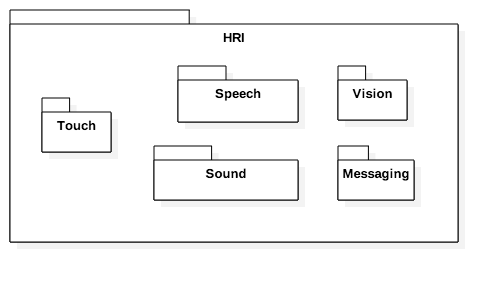
\includegraphics[width=1\linewidth]{imagenes/diagramas/PaquetesGenerales.png}
	\caption{Estructura de paquetes dentro del paquete HRI del Robobo}
	\label{fig:general-package-structure}
\end{figure}

\begin{itemize}
	\item Paquete Speech: Gestiona las operaciones que involucran habla.
		\begin{itemize}
		\item Módulo SpeechProduction: Permite utilizar la síntesis de voz.
		\item Módulo SpeechRecognition: Permite el reconocimiento de voz, por palabras clave o por gramáticas.
		\end{itemize}
	\item Paquete Touch: Gestiona el sentido del tacto del robot.
		\begin{itemize}
		\item Módulo Touch: Permite la detec	ción de gestos en la pantalla táctil del móvil.
		\end{itemize}
	\item Paquete Sound: Gestiona el sentido del oído del robot.
		\begin{itemize}
		\item Módulo SoundDispatcher: Módulo auxiliar para los módulos que emplean la librería TarsosDSP\cite{six2014tarsosdsp}
		\item Módulo ClapDetectionModule: Módulo que permite la detección de sonidos percusivos.
		\item Módulo PitchDetection: Módulo que permite la estimación de la frecuencia de un sonido.
		\item Módulo NoteDetection: Módulo que detecta notas musicales a partir de frecuencias.
		\item Módulo NoteGenerator: Módulo que genera tonos correspondientes a notas musicales.
		\item Módulo Emotionsound: Módulo que permite la reproducción de una serie de sonidos prefijados con el objetivo de expresar sentimientos.
		\end{itemize}
	\item Paquete Vision: Gestiona el sentido de la vista del robot.
	\begin{itemize}
	\item Módulo BasicCamera: Provee de un stream constante de frames capturados desde la cámara frontal del smartphone.
	\item Módulo FaceDetection: Permite detectar caras en los frames capturados por la cámara.
	\item Módulo ColorDetection: Permite detectar colores sobre fondos blancos en los frames.
	
	\end{itemize}
	\item Paquete Messaging: Gestiona los métodos de mensajería del robot
		\begin{itemize}
		\item Módulo Messaging: Permite enviar correos electrónicos, pudiendo adjuntar imágenes.
		\end{itemize}
\end{itemize}


Cada paquete se distribuye en forma de librería Android dentro del paquete HRI del ROBOBO! Framework.

\subsection{Estructura de un módulo}

Todos los módulos comparten una estructura de paquetes similar, un paquete con el nombre del módulo , que contiene la interfaz del módulo (de la forma \textit{INombreModulo}) que extiende la clase \textit{IModule}, una clase abstracta opcional (\textit{ANombreModulo}) que implementa la interfaz anterior y gestiona labores comunes como la suscripción a los Listeners, y los paquetes de las diferentes implementaciones especificas. Opcionalmente, este paquete también podrá contener la interfaz de los listeners, y clases de utilidad como enumerados.

Las implementaciones de los módulos tienen el nombre \textit{NombreImplementacionNombreModulo}, y deben extender la clase abstracta o la interfaz del módulo en caso de carecer de la primera.

\section{Metodología}

La metodología seguida fue un proceso iterativo en el cual en cada iteración se fueron añadiendo nuevos módulos de interacción y realizando correcciones en los módulos ya implementados.
\subsection{Primera iteración}

En esta primera iteración el trabajo de desarrollo se centró en los paquetes de producción y reconocimiento de habla (Paquete \textit{Speech}) y el de tacto (Paquete \textit{Touch}. Se implementaron las funcionalidades básicas de cada módulo:
\begin{itemize}
	\item \textit{SpeechProductionModule}: Se implementaron las funcionalidades de síntesis de voz, selección de voces y de localización.
	\item \textit{SpeechRecognitionModule}: Se implementó el reconocimiento básico por palabras clave.
	\item \textit{TouchModule}: Se implementaron el reconocimiento de toques largos(touch) y cortos(tap), así como el reconocimiento de caricias(caress) y deslizamientos rápidos(fling).
\end{itemize} 

\subsection{Segunda iteración}
En la segunda iteración se desarrolló el paquete de interacción por sonidos y se realizaron correcciones tanto en el módulo de reconocimiento de voz cómo en el táctil.

Nuevas implementaciones en esta iteración:

\begin{itemize}
	\item \textit{SoundDispatcherModule}: Implementado para dar soporte al resto de módulos que usan la librería TarsosDSP\cite{six2014tarsosdsp}.
	\item \textit{ClapDetectionModule}: Implementado el módulo de detección de sonidos percusivos.
	\item \textit{PitchDetectionModule}: Implementada el módulo de detección de frecuencias en hertzios.
	\item \textit{NoteDetectionModule}: Implementada el módulo de detección de notas musicales. Implementada clase para representar las notas.
\end{itemize}

Actualizaciones de módulos de la anterior iteración:

\begin{itemize}
	\item \textit{SpeechRecognitionModule}: Implementada la búsqueda por gramáticas
	\item \textit{TouchModule}: Mejorada la información producida por el evento \textit{onFling}.
\end{itemize}

\subsection{Tercera iteración}

En esta iteración se desarrollaron los paquetes de visión y de mensajería. También se sacaron de dentro de los módulos los diferentes parámetros, para poder ser configurados desde el exterior mediante ficheros \textit{properties}.

Nuevas implementaciones en esta iteración:

\begin{itemize}
	\item \textit{BasicCameraModule}: Implementado el notificador de frames.
	\item \textit{FaceDetectionModule}: Implementado el modulo de detección de caras.
	\item \textit{ColorDetectionModule}: Implementado el modulo de detección de colores.
	\item \textit{MessagingModule}: Implementado el módulo de mensajería por gMail.
\end{itemize}

Actualizaciones de módulos:

\begin{itemize}
	\item \textit{SoundDispatcherModule}: Parametrización mediante properties.
	\item \textit{ClapDetectionModule}: Parametrización mediante properties.
	\item \textit{PitchDetectionModule}: Parametrización mediante properties.

\end{itemize}

\subsection{Cuarta iteración}

En esta iteración se añadieron dos módulos de producción de sonidos.


Nuevas implementaciones esta iteración:
\begin{itemize}
	\item \textit{EmotionSoundModule}: Implementada la reproducción de sonidos prefijados.
	\item \textit{NoteGeneratorModule}: Implementada la generación de tonos.
\end{itemize}

Actualizaciones de módulos:

\begin{itemize}
	\item \textit{ColorDetectionModule}: Añadida una comprobación de la varianza del color para evitar falsos positivos.
\end{itemize}
\newpage

\section{Librerías de interacción}
A continuación se hablará sobre los detalles de implementación de las diferentes librerías de interacción desarrolladas.
\label{sec:InteractionLibraries}

%%%%%%%%%%%%%%%%%%%%%%%%%%%%%%%%%%%%%%%%%%%%%%%%%%%%%%%%%%%%%%%%%%%%%%%%%%%%%%%%
\subsection{Paquete Speech}
\label{subsec:speech-package}
Este subsistema gestiona todas las labores que tienen que ver con la generación o detención del habla. En su interior encapsula dos paquetes diferentes (figura \ref{fig:speech-package}) , Production y Recognition, que contienen respectivamente los módulos de producción y reconocimiento del habla.
\begin{figure}
	\centering
	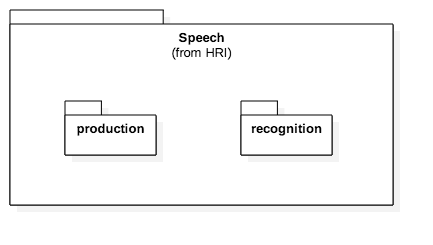
\includegraphics[width=0.8\linewidth]{imagenes/diagramas/Speech.png}
	\caption{Paquete Speech}
	\label{fig:speech-package}
\end{figure}

%%%%%%%%%%%%%%
\subsubsection{Módulo recognition}
\begin{figure}
	\centering
	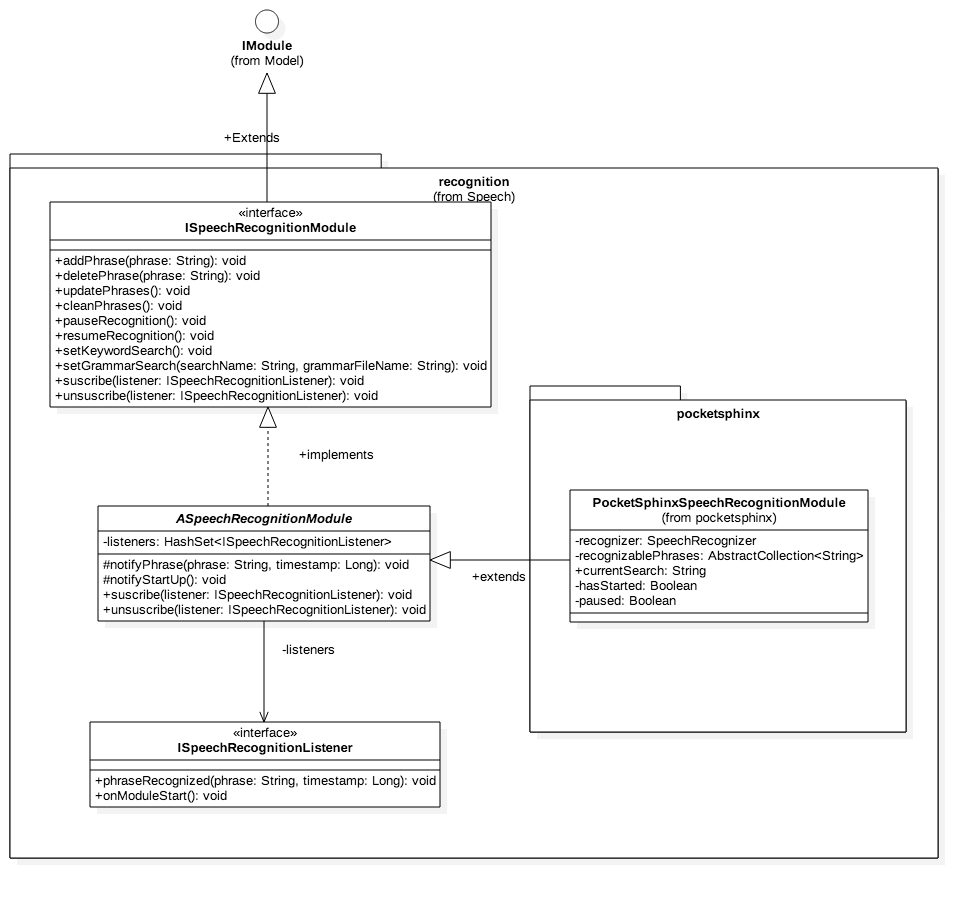
\includegraphics[width=1\linewidth]{imagenes/diagramas/SpeechRecognitionModule.png}
	\caption{Módulo SpeechRecognition}
	\label{fig:speech-recognition-module}
\end{figure}
El módulo recognition(figura \ref{fig:speech-recognition-module}) permite al usuario reconocer texto hablado de forma fácil.
Provee las Interfaces \textit{ISpeechRecognitionModule} y \textit{ISpeechRecognitionListener}, así cómo la clase abstracta \textit{ASpeechRecognitionModule}.


\textit{ISpeechRecognitionModule} ofrece la declaración de métodos de configuración del reconocedor de  voz y de suscripción de listeners.


Esta interfaz proporciona funcionalidades de:
\begin{itemize}
 	\item Añadir y eliminar palabras reconocibles.
 	\item Actualizar el listado interno de frases
	\item Limpiar el listado interno
	\item Pausar y reanudar el reconocimiento
	\item Añadir búsquedas por gramática
	\item Utilizar búsqueda por palabras
 	 
\end{itemize}



\textit{ISpeechRecognitionListener} es la interfaz que deben implementar las clases para ser notificados de los eventos que produce el módulo de reconocimiento.

Las clases suscritas este listener son notificadas cuando:
\begin{itemize}
	\item El reconocedor ha sido inicializado
	\item Una frase ha sido detectada
\end{itemize}

   


\textit{ASpeechRecognitionModule} es la clase abstracta que gestiona las tareas comunes a todas las implementaciones del modulo, a saber:

\begin{itemize}
	\item Mantener un listado de los listeners
	\item Suscribir y desuscribir listeners
	\item Notificar a los listeners de los diferentes eventos
\end{itemize}





\paragraph*{Pocketsphinx\\}


Se ha decidido realizar la implementación del módulo utilizando la librería CMU Sphinx \cite{cmusphinx}, desarrollada por la Universidad de Carnegie Mellon que se ha presentado en la sección \ref{subsec:sphinx}.
Específicamente se utiliza PocketSphinx, una versión de CMU Sphinx ligera, diseñada para su uso en sistemas embebidos.

PocketSphinx permite varios tipos de búsqueda diferentes, pero al contrario que las versiones más completas de la librería, sólo permite tener una búsqueda activa al mismo tiempo.

Entre los modos de búsqueda que ofrece se encuentran la búsqueda por Keywords y la búsqueda por Gramáticas, que son las que son ofrecidas por la interfaz del módulo. Adicionalmente PS también permite el uso de búsquedas por fonemas, pero no se ha contemplado su uso.

El módulo se llama  \textit{PocketSphinxSpeechRecognitionModule}, extiende \textit{ASpeechRecognitionModule} e implementa la interfaz \textit{RecognitionListener} que provee PocketSphinx.

La búsqueda por keywords permite al usuario definir, en tiempo de ejecución, una serie de palabras que podrán ser reconocidas, estas palabras deben estar contenidas en el diccionario del modelo fonético.

La búsqueda por gramática permite definir archivos de gramáticas en el formato  JSFG 1.0\cite{JSFGGrammar}, lo cual permite detectar construcciones más complejas de palabras.
%%todo Esto debería ir en el manual de usuario?
Para funcionar correctamente deben colocarse en el directorio assets/sync/ de la aplicación tanto el modelo fonético del idioma, como los archivos de gramáticas que se vayan a utilizar, todo archivo dentro de este directorio debe contar con un fichero de mismo nombre y extensión .md5 conteniendo un hash del original en su interior. Los archivos deben ser declarados dentro del fichero assets.lst.

Dado que el inicio del reconocedor de voz se realiza de manera asíncrona, es necesario notificar a la aplicación principal de cuando el módulo esta preparado, de lo contrario, llamar a una operación del mismo podría ser inseguro. Le arranque del módulo se notifica a través del método onModuleStart() que debe ser implementado por cualquier clase que vaya a utilizar el  módulo.

%%%%%%%%%%%%%%
\subsubsection{Módulo Production}

\begin{figure}
	\centering
	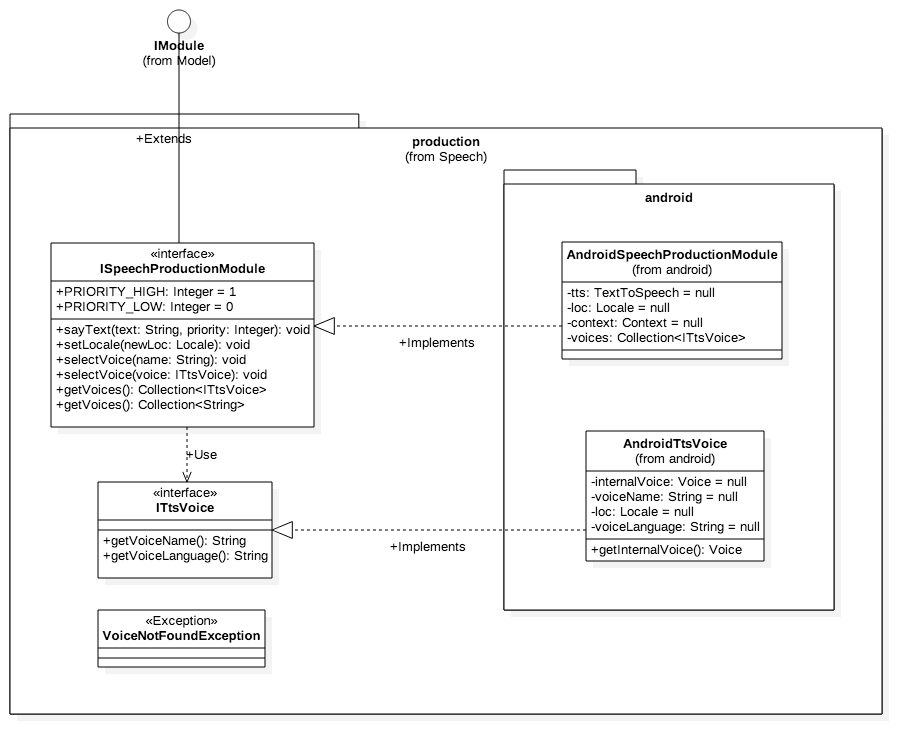
\includegraphics[width=1\linewidth]{imagenes/diagramas/SpeechProductionModule.png}
	\caption{Módulo SpeechProduction}
	\label{fig:speech-production-module}
\end{figure}




El módulo production(figura \ref{fig:speech-production-module}) permite al usuario producir voz a partir de texto de manera simple.
Provee la interfaces \textit{ISpeechProductionModule} y \textit{ITtsVoice}, así como la excepción \textit{VoiceNotFoundException}.
La primera contiene las declaraciones de los métodos del módulo en sí, la segunda proporciona una forma de representar las diferentes voces a utilizar por el módulo.

Las funcionalidades que facilita la interfaz son:

\begin{itemize}
	\item Pronunciar un texto
	\item Cambiar la localización 
	\item Seleccionar voces
	\item Recuperar las voces disponibles
\end{itemize}

 


Implementación específica:

La implementación de la interfaz se ha realizado con las librerías del propio sistema Android (\textbf{android.speech.tts.TextToSpeech})

\subsubsection*{Ejemplos de desarrollo}

Para la prueba de los módulos de voz se realizaron dos ejemplos básicos, una aplicación simple en la que el usuario introduce un texto y el teléfono lo pronuncia, y un sistema de control mediante voz en el que el usuario le daba ordenes básicas al Robobo mediante la voz y este, al terminar la frase, ejecutaba los movimientos indicados.
A continuación se puede observar una muestra del log de la aplicación de control por voz:

\begin{verbatim}
D/SpeechRecognitionModule: Recognized part rob
D/SpeechRecognitionModule: Recognized part rob front
D/SpeechRecognitionModule: Recognized part rob front now
I/SpeechRecognizer: Stop recognition
D/SpeechRecognitionModule: Recognized rob front now Prob: -4730
D/SpeechROB: rob front now
D/ROB-INTERFACE: Move forwards: 50 - 360
I/SpeechRecognizer: Start recognition "MovSearch"
D/SpeechRecognizer: Starting decoding
\end{verbatim}

En este log se puede ver cómo el reconocedor detecta las tres partes de la frase, detiene el reconocimiento al detectar una frase válida en la gramática, se ejecuta un movimiento a través del módulo \textit{Rob-Interface} y se reanuda la escucha.
En el siguiente fragmento de código se puede ver la implementación del listener del reconocedor de frases.
\begin{lstlisting}
	 @Override
    public void phraseRecognized(final String phrase, Long timestamp) {
        try {
            Log.d("SpeechROB",phrase);
            if (phrase.equals("rob up now")) {
                movementModule.moveTilt(90);
            }
            if (phrase.equals("rob down now")) {
                movementModule.moveTilt(45);
            }
            if (phrase.equals("rob left now")) {
                movementModule.turnLeftAngle((short) 50, 360);
            }
            if (phrase.equals("rob right now")) {
                movementModule.turnRightAngle((short) 50, 360);
            }
            if (phrase.equals("rob front now")) {
                movementModule.moveForwardsAngle((short) 50, 360);
            }
            if (phrase.equals("rob back now")) {
                movementModule.moveBackwardsAngle((short) 50, 360);
            }
        } catch (InternalErrorException e){
        }
        runOnUiThread(new Runnable() {
            @Override
            public void run() {
                textView.setText(phrase);
            }
        });
    }
\end{lstlisting}
\newpage
%%%%%%%%%%%%%%%%%%%%%%%%%%%%%%%%%%%%%%%%%%%%%%%%%%%%%%%%%%%%%%%%%%%%%%%%%%%%%%%%%
\subsection{Paquete Touch}


\begin{figure}
	\centering
	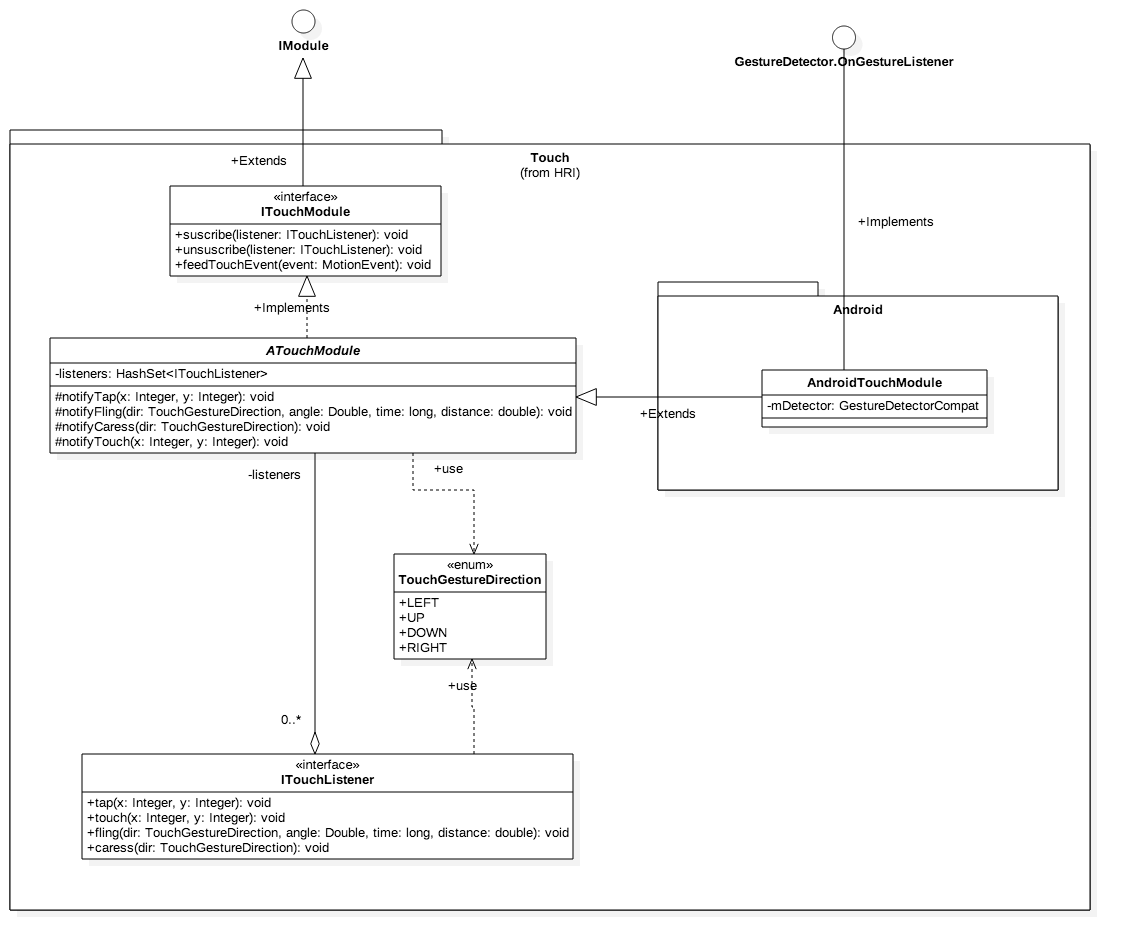
\includegraphics[width=1\linewidth]{imagenes/diagramas/TouchModule.png}
	\caption{Módulo Touch}
	\label{fig:touch-module}
\end{figure}


El subsistema Touch permite interacción con el robot en forma de gestos táctiles sobre la pantalla del teléfono. En su interior encontramos un único modulo, el módulo touch.
%%%%%%%%%%%%%%
\subsubsection{Módulo Touch}
El módulo(figura \ref{fig:touch-module}) contiene las interfaces \textit{ITouchModule} e \textit{ITouchListener}, la clase abstracta \textit{ATouchModule} y por la clase enumerado \textit{TouchGestureDirection}.

\textit{ITouchListener} es la interfaz que debe implementar cualquier clase que quiera ser informada de los gestos táctiles que ocurran en la pantalla del dispositivo. Las acciones que se detectan son:

\begin{itemize}
	\item  Tap: Toque simple y rápido en la pantalla
	\item  Touch: Toque mantenido en la pantalla
	\item  Caress: Deslizamiento sobre la pantalla
	\item  Fling: Al terminar un deslizamiento de manera rápida
\end{itemize}


\textit{ITouchModule} es la interfaz que debe implementar cualquier implementación del módulo. El único método destacado de la misma es \textit{FeedTouchEvent}, en el cual se le pasan los eventos táctiles al módulo desde la aplicación principal, que debe sobrecargar el método \textit{OnTouchEvent} de la clase \textit{Activity}, esto es debido a que el módulo no puede extender la clase \textit{Activity}.

\paragraph*{Detección táctil de Android\\}


Para la implementación del módulo se escogió usar la clase \textit{GestureDetector} propia de Android, que provee de varios listeners para diferentes eventos táctiles.
Se han simplificado dichos eventos, para producir los definidos en \textit{ITouchListener}

\subsubsection*{Ejemplos de desarrollo}

Se implementó una simple aplicación que mostraba por pantalla los diferentes eventos producidos por el módulo \textit{TouchModule}.
 A continuación se ve la implementación del listener \textit{fling} en el ejemplo anterior:
 
 \begin{lstlisting}
 	@Override
    public void fling(TouchGestureDirection dir, double angle, long time, double distance) {
        speechProductionModule.sayText("Fling",ISpeechProductionModule.PRIORITY_HIGH);
        Log.d(TAG,"FLING");
        textView.setText("FLING: "+dir.toString()+" Time: "+time+" Distance: "+distance+" Angle: "+Math.toDegrees(angle));
    }
 \end{lstlisting}


\newpage

%%%%%%%%%%%%%%%%%%%%%%%%%%%%%%%%%%%%%%%%%%%%%%%%%%%%%%%%%%%%%%%%%%%%%%%%%%%%%%%%
\subsection{Paquete Sound}
Este subsistema contiene los módulos(figura \ref{fig:sound-package} que realizan diversas tareas de reconocimiento y producción de audio.  Han sido implementadas tanto detección de tonos, notas musicales y palmadas, como síntesis de notas musicales y producción de sonidos prefijados.
\begin{figure}
	\centering
	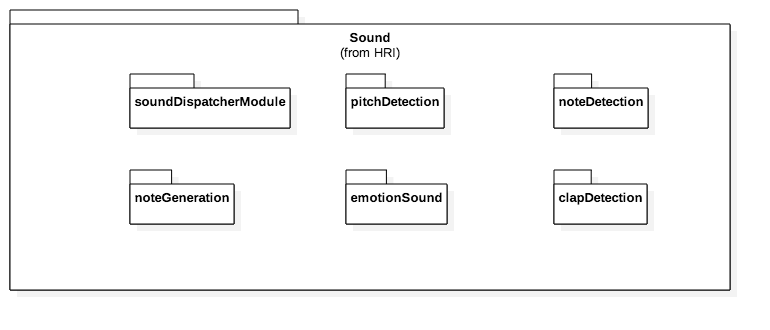
\includegraphics[width=1\linewidth]{imagenes/diagramas/Sound.png}
	\caption{Paquete Sound}
	\label{fig:sound-package}
\end{figure}
%%%%%%%%%%%%%%
\subsubsection{Módulo Sound Dispatcher}
\begin{figure}
	\centering
	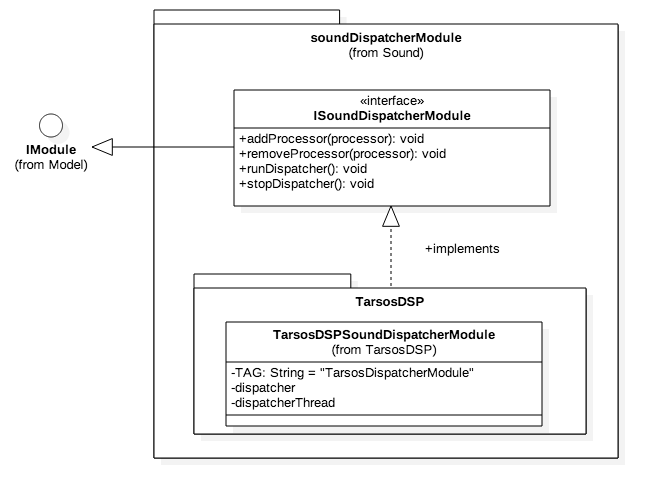
\includegraphics[width=1\linewidth]{imagenes/diagramas/SoundDispatcherModule.png}
	\caption{Módulo SoundDispatcher}
	\label{fig:sound-dispatcher-module}
\end{figure}
SoundDispatcher(figura \ref{fig:sound-dispatcher-module}) es un módulo de utilidad, necesario para el uso de los módulos implementados a partir de la librería TarsosDSP \cite{six2014tarsosdsp}.
Este módulo es el que se encarga de capturar el sonido del micrófono y segmentarlo en partes para su posterior procesado. Los distintos módulos se registran con sus procesadores en este módulo.
El paquete contiene en su interior \textit{ISoundDispatcherModule}, la interfaz del módulo, que permite
\begin{itemize}
	\item Añadir procesadores de audio
	\item Eliminar procesadores de audio
	\item Iniciar el procesado de audio
	\item Parar el procesado de audio
\end{itemize}

\paragraph*{TarsosDSP\\}
La implementación se realiza en el módulo \textit{TarsosDSPSoundDispatcherModule}, que implementa la interfaz \textit{ISoundDispatcherModule}.
En su interior se crea un objeto \textit{AudioDispatcher}, que se encarga del procesado del audio, y al que pueden añadirse distintos procesadores de audio.

Los parámetros del objeto soundDispatcher pueden indicarse en el archivo sound.properties, pudiendo fijar el la tasa de muestreo(samplerate), el tamaño del buffer(buffer) y el solapado entre ventanas de audio(overlap).

%%%%%%%%%%%%%%
\subsubsection{Módulo Pitch Detection}
\begin{figure}
	\centering
	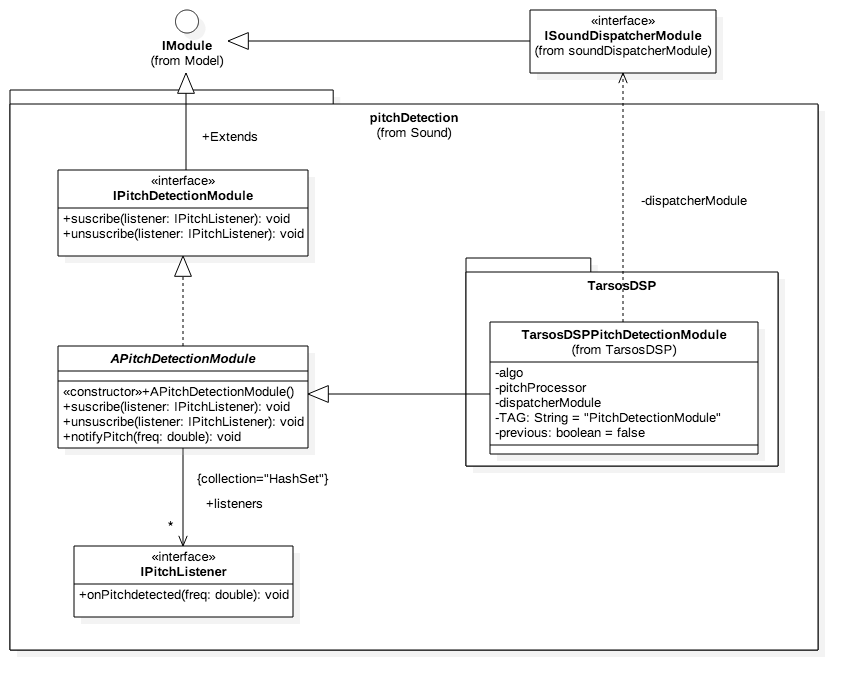
\includegraphics[width=1\linewidth]{imagenes/diagramas/PitchDetectionModule.png}
	\caption{Módulo PitchDetection}
	\label{fig:pitch-detection-module}
\end{figure}
PitchDetection(figura \ref{fig:pitch-detection-module}) permite detectar la frecuencia en Hertzios de sonidos, es utilizado, por ejemplo en el módulo de detección de notas musicales.
En su interior encontramos la interfaz \textit{IPitchDetectionModule} y la clase abstracta \textit{APitchDetectionModule}, que gestionan la suscripción de listeners a los eventos. También se encuentra \textit{IPitchListener}, que debe ser implementada por cualquier clase que desee recibir notificaciones del módulo de detección de tonos.

\paragraph*{TarsosDSP \\}
La implementación del módulo se ha realizado en la clase \textit{TarsosDSPPitchDetectionModule}. Esta implementación depende del módulo SoundDispatcher, ya que en su inicialización se registra a su procesador de audio en el soundDispatcher.
%TODO No se muy bien como redactar esto
Esta implementación utiliza el algoritmo YIN \cite{de_YINa_f2002} para la detección de frecuencias. La implementación del algoritmo viene dada por la propia librería TarsosDSP. El módulo genera un evento con la frecuencia cuando un sonido es detectado, y al terminar la detección devuelve un -1.

%%%%%%%%%%%%%%
\subsubsection{Módulo Note Detection}
\begin{figure}
	\centering
	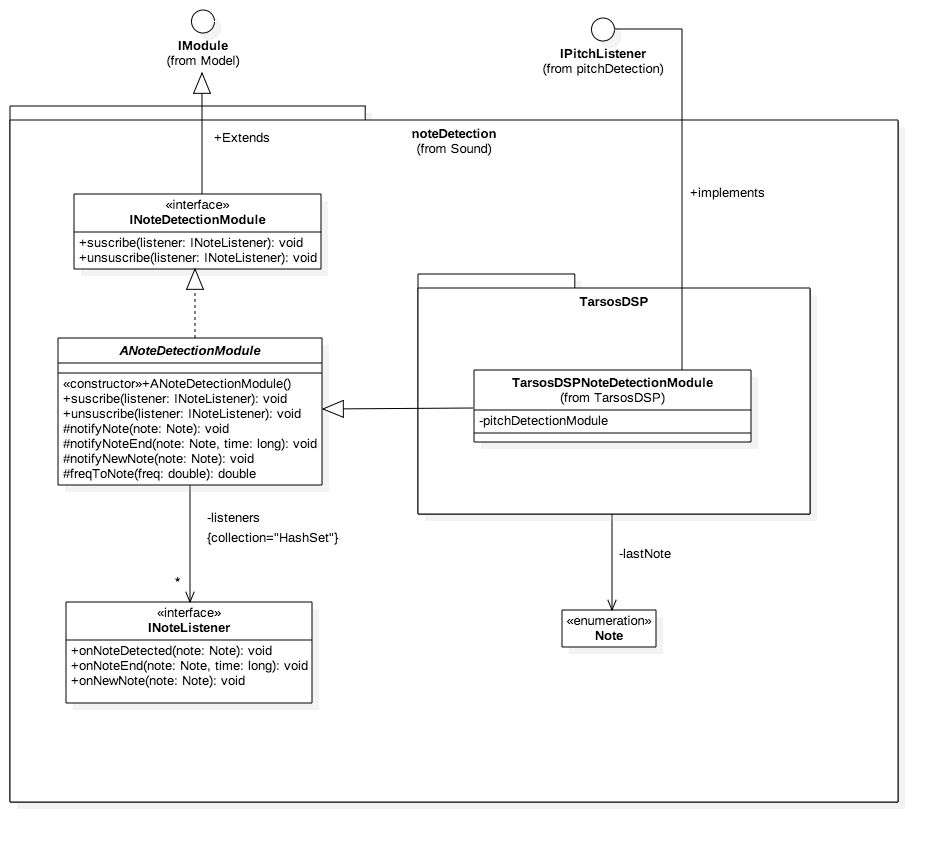
\includegraphics[width=1\linewidth]{imagenes/diagramas/NoteDetectionModule.png}
	\caption{Módulo NoteDetection}
	\label{fig:note-detection-module}
\end{figure}
El módulo NoteDetection(figura \ref{fig:note-detection-module}) busca proporcionar una manera simple de detectar notas musicales. Depende directamente del módulo PitchDetection, del cual obtiene la frecuencia que traduce en notas musicales.
En su interior encontramos la interfaz del módulo \textit{INoteDetectionModule}, la clase abstracta \textit{ANoteDetectionModule}, que además de la gestión de listeners provee un método de conversión de frecuencias a notas, la interfaz \textit{INoteListener} que recibe notificaciones al:
\begin{itemize}
	\item Comenzar una nota
	\item Detectar una nota
	\item Terminar una nota
\end{itemize}
 Toda clase que desee recibir los eventos producidos por el módulo debe implementar esta interfaz.
 Por último en el paquete encontramos una clase \textit{Note} que se utiliza como representación de las notas musicales. Este enumerado contiene la información del índice de la conversión de notas, la nota musical en formato anglosajón, y la octava a la que pertenece la nota.
 
 \paragraph*{TarsosDSP\\}%todo realmente no usa la libreria directamente
 
 \textit{TarsosDSPNoteDetectionModule} extiende \textit{ANoteDetectionModule} e implementa \textit{IPitchListener}. Simplemente convierte los tonos detectados a notas musicales, filtra las notas desafinadas(descarta las que se desvían un 10\% respecto al indice) y controla los inicios y finalizaciones de las notas, generando eventos de los cuales serán notificados los listeners.
 
%%%%%%%%%%%%%%
\subsubsection{Módulo Clap Detection}
\begin{figure}
	\centering
	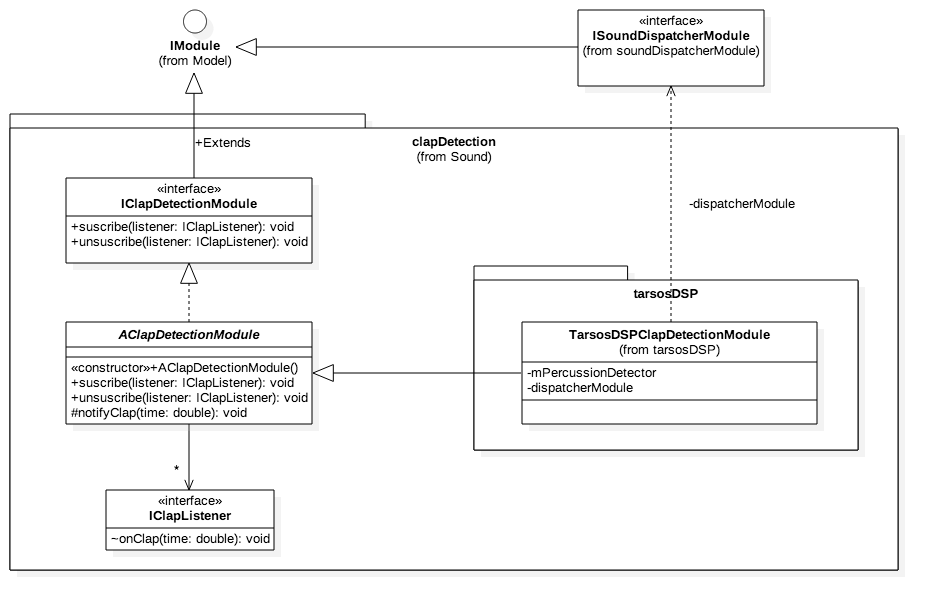
\includegraphics[width=1\linewidth]{imagenes/diagramas/ClapDetectionModule.png}
	\caption{Módulo ClapDetection}
	\label{fig:clap-detection-module}
\end{figure}
El módulo ClapDetection(figura \ref{fig:clap-detection-module}) permite detectar ruidos percusivos tales como palmadas. Igual que el PitchDetection, depende directamente del módulo SoundDispatcher para su funcionamiento. En su interior se encuentra la interfaz del módulo, \textit{IClapDetectionModule}, la clase abstracta \textit{AClapDetectionModule} y la interfaz del listener, \textit{IClapListener}. Las clases que implementen este listener recibirán una notificación cada vez que se detecte una palmada.
\paragraph*{TarsosDSP\\} 
La implementación del módulo, contenida en \textit{TarsosDSPClapDetectionModule}, emplea el objeto provisto por la librería TarsosDSP \textit{PercussionOnsetDetector}, que es registrado en el \textit{DispatcherModule} activo en ese momento. Este objeto permite la detección de sonidos percusivos, como palmadas, de una forma sencilla.

%%%%%%%%%%%%%%
\subsubsection{Módulo NoteGenerator}
\begin{figure}
	\centering
	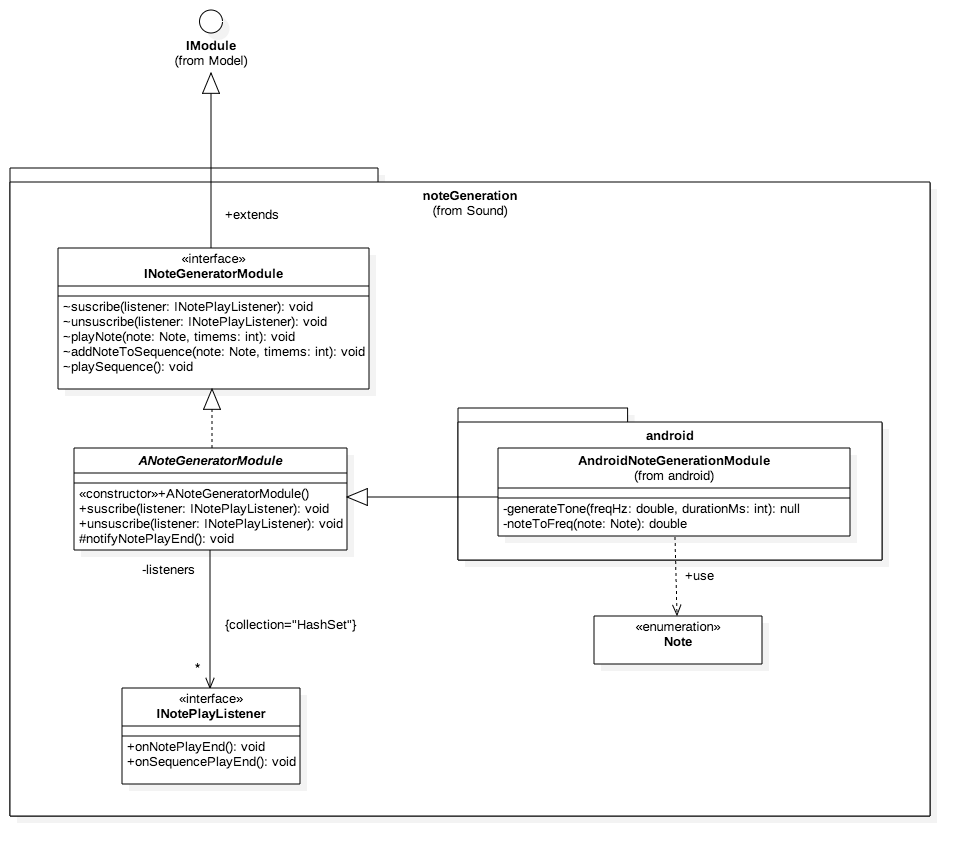
\includegraphics[width=1\linewidth]{imagenes/diagramas/NoteGenerationModule.png}
	\caption{Módulo NoteGenerator}
	\label{fig:note-generator-module}
\end{figure}
El módulo NoteGenerator(figura \ref{fig:note-generator-module}) provee una forma de sintetizar tonos musicales y reproducir secuencias de notas.
En su interior se encuentra la interfaz del módulo \textit{INoteGeneratorModule} que define las funcionalidades del módulo y la clase abstracta \textit{ANoteGeneratorModule} que gestiona la suscripción a los listeners. La interfaz del listener se encuentra en \textit{INotePlayListener} y su finalidad es notificar cuando una nota o una secuencia de notas termina de reproducirse. La clase \textit{Note} es la representación de las notas musicales en el sistema, contiene la nota, el índice y la octava.

\paragraph*{Android\\}

La implementación especifica del módulo se encuentra en \textit{AndroidNoteGeneratorModule} y se ha realizado mediante la clase \textit{AudioTrack} proporcionada por la API de Android. El objeto \textit{AudioTrack} se crea sample a sample utilizando la ecuación de una onda senoidal de la frecuencia de la nota requerida. La reproducción de secuencias se implementa mediante el uso de las clases \textit{Timer} y \textit{TimerTask}

%%%%%%%%%%%%%%
\subsubsection{Módulo EmotionSound}
\begin{figure}
	\centering
	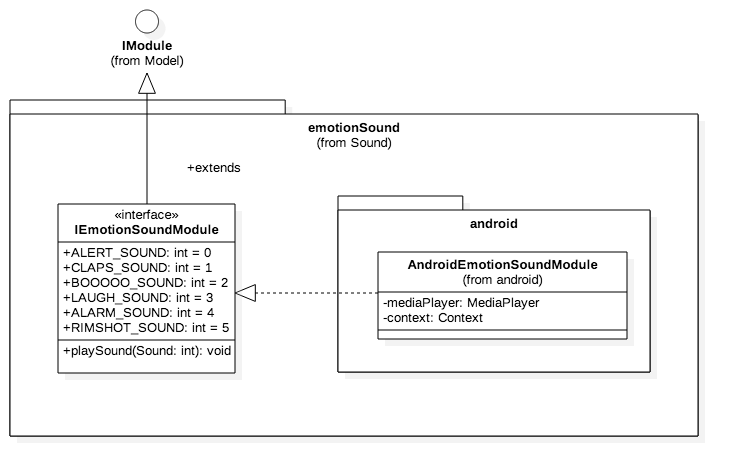
\includegraphics[width=1\linewidth]{imagenes/diagramas/EmotionSoundModule.png}
	\caption{Módulo EmotionSound}
	\label{fig:emotion-sound-module}
\end{figure}
El módulo EmotionSound(figura \ref{fig:emotion-sound-module}) busca proporcionar una manera de reproducir una serie de sonidos prefijados para expresar diferentes emociones.
La interfaz del módulo esta definida en \textit{IEmotionSoundModule}, y en ella se declaran, en forma de constantes, los sonidos utilizables.
Los sonidos se encuentran en el directorio /raw de la carpeta /res del paquete Sound.

\paragraph*{Android\\}

La implementación de este módulo se ha realizado mediante la clase \textit{MediaPlayer} provista por la API de Android, que permite reproducir diferentes recursos audiovisuales. El módulo está definido en la clase \textit{AndroidEmotionSoundModule}.


\subsubsection*{Ejemplos de desarrollo}

Para probar la detección de notas musicales se desarrolló un control mediante música en el que el usuario ejecutaba una secuencia de notas musicales en una escala, cada una correspondiendo a una acción de movimiento, y al recibir la nota de cierre de secuencia, el ROBOBO ejecutaba los movimientos indicados. A continuación se muestra un ejemplo de log de la ejecución:

\begin{verbatim}
D/MusicActivity: Note: A
D/MusicActivity: recording
D/MusicActivity: Note: As
D/MusicActivity: Note: D
D/MusicActivity: adding command
D/MusicActivity: Note: Ds
D/MusicActivity: Note: E
D/MusicActivity: adding command
D/MusicActivity: Note: G
D/MusicActivity: adding command
D/MusicActivity: Note: A
D/MusicActivity: executing
D/MusicActivity: Executing command $NoteCommand@14bb8f87
D/ROB-INTERFACE: Move backwards: 60 - 861
D/MusicActivity: Executing command $NoteCommand@3016eb4
D/ROB-INTERFACE: Turn left: 60 - 1816
D/MusicActivity: Executing command $NoteCommand@a8f2add
D/ROB-INTERFACE: Turn right: 60 - 1816
\end{verbatim} 

Se puede ver como la nota A(La) abre la secuencia de comandos, As(La sostenido) y Ds(Re sostenido) son ignorados al no estar en la escala definida (A, C, D, E, G), son añadidos tres comandos de movimiento (Correspondientes a las notas D(Re), E(Mi) y G(Sol)) y la nota A cierra la secuencia de comandos que serán ejecutados a través de la \textit{Rob-Interface}.


A continuación se muestra la implementación del listener \textit{onNoteEnd} usada en el módulo anterior:

\begin{lstlisting}
	 @Override
    public void onNoteEnd(Note note, long time) {
        Log.d(TAG,"Note: "+note.note);
        if (!executing) {
            if (note.note == (triggerNote)) {
                if ((recording)&&(time>100)) {
                    recording = false;
                    executing = true;
                    Log.d(TAG,"executing");
                    runOnUiThread(new Runnable() {
                        @Override
                        public void run() {
                            rellayout.setBackgroundColor(Color.BLUE);
                        }
                    });
                    executeCommands(commandList);
                } else {
                    Log.d(TAG,"recording");
                    recording = true;
                    runOnUiThread(new Runnable() {
                        @Override
                        public void run() {
                           rellayout.setBackgroundColor(Color.GREEN);
                        }
                    });
                }
            } else {
                if (recording) {
                    if (scale.contains(note.note)) {
                        Log.d(TAG,"adding command");
                        commandList.add(new NoteCommand(note, time));
                    } else {
                        //Bad note
     }}}}}
\end{lstlisting}



\newpage
%%%%%%%%%%%%%%%%%%%%%%%%%%%%%%%%%%%%%%%%%%%%%%%%%%%%%%%%%%%%%%%%%%%%%%%%%%%%%%%%
\subsection{Paquete Vision}
Este subsistema(figura \ref{fig:vision-package}) contiene los diferentes módulos de captura y procesado de imagen

\begin{figure}
	\centering
	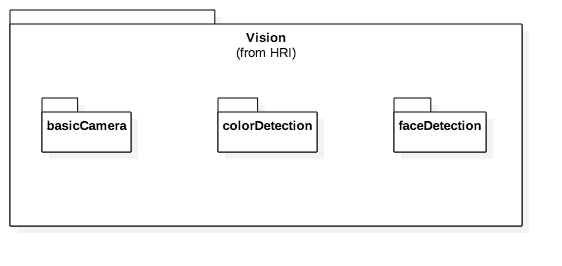
\includegraphics[width=0.8\linewidth]{imagenes/diagramas/Vision.png}
	\caption{Paquete Vision}
	\label{fig:vision-package}
\end{figure}

%%%%%%%%%%%%%%
\subsubsection{Módulo Basic Camera}
\begin{figure}
	\centering
	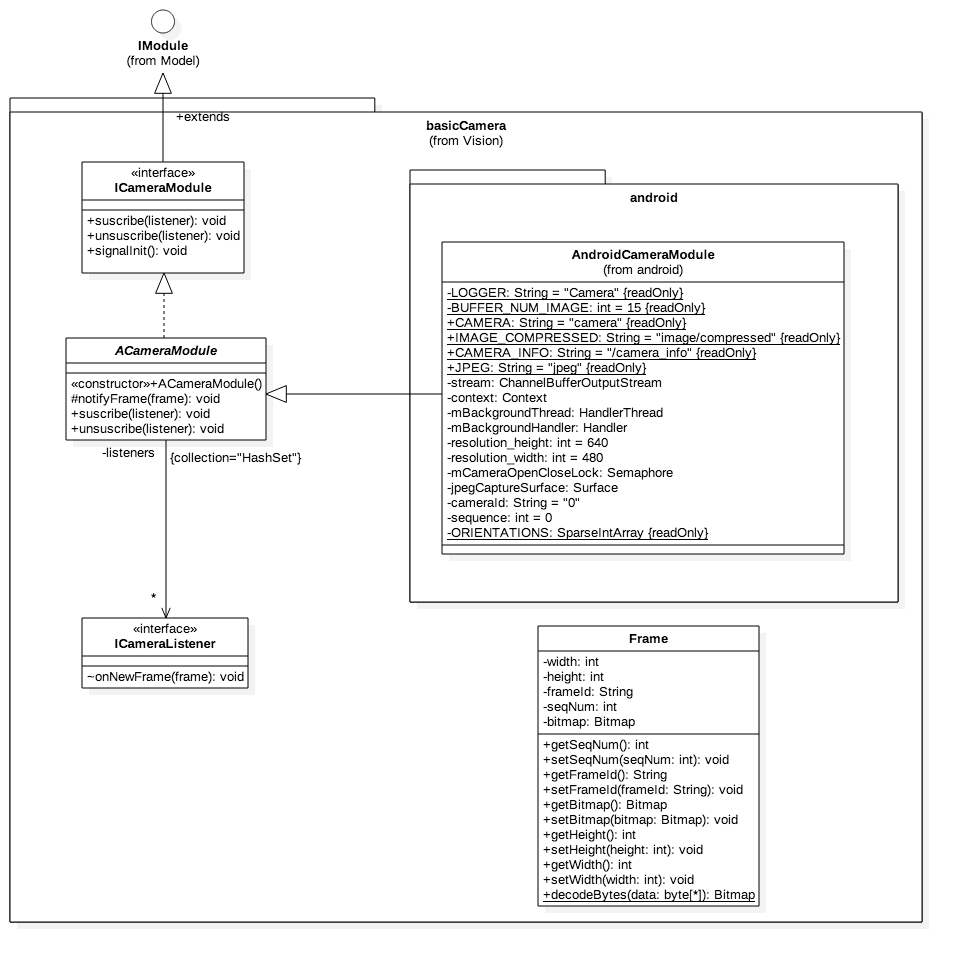
\includegraphics[width=1\linewidth]{imagenes/diagramas/BasicCameraModule.png}
	\caption{Módulo BasicCamera}
	\label{fig:basic-camera-module}
\end{figure}
Este es el módulo básico de cámara(figura \ref{fig:basic-camera-module}) , del cual hacen uso el resto de módulos de procesado de imagen. Este modulo produce un stream constante de imágenes capturadas de la cámara frontal del dispositivo y notifica a los listeners suscritos.
La interfaz del módulo se encuentra en \textit{ICameraModule}, la clase abstracta que gestiona los listeners en \textit{ACameraModule} y la interfaz del listener en el que se notifica la captura de las imágenes en \textit{ICameraListener}. Además, el modulo proporciona una clase Frame, que representa a las imágenes capturadas con sus características.

\paragraph*{Android Camera2\\}
Para realizar la implementación del módulo se ha empleado la clase \textit{Camera2} que proporciona Android. Esta implementación permite obtener el stream mencionado anteriormente sin mostrar las imágenes en la pantalla, pero produce una velocidad de captura de imágenes baja, de alrededor de dos cuadros por segundo en el smartphone de pruebas (BQ Aquaris M5) variando de teléfono a teléfono.

%%%%%%%%%%%%%%
\subsubsection{Módulo Face Detection}
\begin{figure}
	\centering
	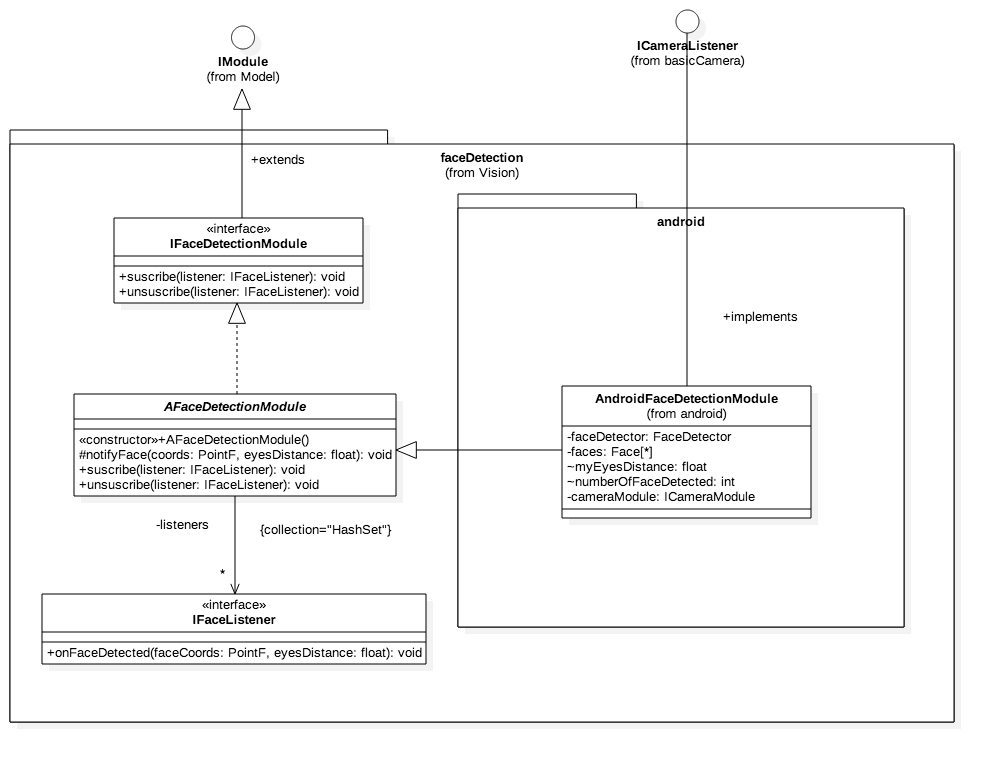
\includegraphics[width=1\linewidth]{imagenes/diagramas/FaceDetectionModule.png}
	\caption{Módulo FaceDetection}
	\label{fig:face-detection-module}
\end{figure}
El módulo FaceDetection(figura \ref{fig:face-detection-module}) permite detectar caras en los frames producidos por el módulo BasicCamera. La interfaz del módulo es \textit{IFaceDetectionModule} y su clase abstracta \textit{AFaceDetectionModule}. El listener que debe ser implementado por la clase que utilice el módulo es \textit{IFaceListener}, que notifica de las coordenadas del centro de la cara y de la distancia entre ojos cuando una cara es detectada. Solo se contempla la detección de una cara al mismo tiempo.

\paragraph*{Android FaceDetector\\}
Para implementar este módulo se ha empleado la clase \textit{FaceDetector} provista por el paquete Media de Android, el módulo se llama \textit{AndroidFaceDetectionModule}.
\newpage

%%%%%%%%%%%%%%
\subsubsection{Módulo ColorDetector}
\begin{figure}
	\centering
	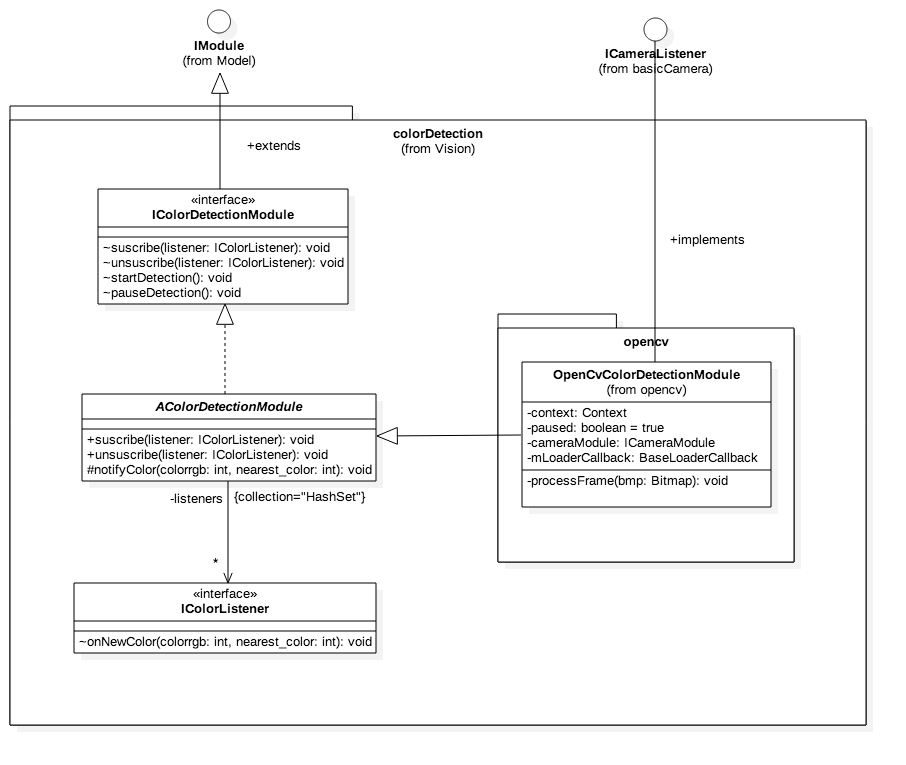
\includegraphics[width=1\linewidth]{imagenes/diagramas/ColorDetectionModule.png}
	\caption{Módulo ColorDetection}
	\label{fig:color-detection-module}
\end{figure}
Este módulo(figura \ref{fig:color-detection-module}) provee la funcionalidad de detección de colores sobre fondos con alto contraste. La interfaz del módulo se puede encontrar en \textit{IColorDetectionModule}, la clase abstracta \textit{AColorDetectionModule} gestiona los listeners en los que será notificada la detección de los colores. La interfaz de dicho listener se encuentra en la clase \textit{IColorListener} y debe ser implementada por toda clase que desee recibir las notificaciones de los colores.

\paragraph*{OpenCV\\}

Para realizar la implementación de este módulo se ha empleado la librería OpenCV\cite{itseez2015opencv} (sección \ref{subsec:opencv}) una de las más usadas en visión por computador. Este módulo, contenido en \textit{OpenCVColorDetectionModule} realiza los siguientes pasos para la detección de colores:
\begin{itemize}
	\item Detección de bordes mediante el algoritmo de Canny, obteniendo el contorno con mayor area.
	\item Creación de una máscara binaria con el área detectada
	\item Conversión de la imagen original al espacio de color HSV
	\item Media de color en los pixeles no nulos en el canal H de la imagen resultante de un AND entre la máscara y la imagen convertida
	\item Filtrado por la varianza del color, si supera 1.1 es descartado
	\item Clasificación del color detectado
\end{itemize}
%%%%%%%%%%%%%%

\subsubsection*{Ejemplos de desarrollo}

Se desarrolló una aplicación que podría considerarse el primer prototipo del ejemplo \textit{ROBOBO Vigilante}(sección \ref{subsec:robobo-vigilante}) que cuando detectaba una cara en la imagen capturada por la cámara mandaba un mensaje por correo electrónico al usuario adjuntando la imagen, se puede ver un ejemplo de este mensaje en la figura \ref{fig:mail-example}.
A continuación se muestra la implementación del listener de caras del ejemplo:

\begin{lstlisting}
	    @Override
    public void onFaceDetected(PointF faceCoords, float eyesDistance) {
        if ((System.currentTimeMillis()-lastDetection)>10000) {
            lastDetection = System.currentTimeMillis();
            msgModule.sendMessage("FACE DETECTED", "xxxxxxxxxx@gmail.com", actualFrame.getBitmap());
        }}
\end{lstlisting}


Para probar el módulo de detección de color se programó una pequeña aplicación que cambiaba el color de fondo de la pantalla acorde al color detectado por el módulo(figuras \ref{fig:blue_color},\ref{fig:cyan_color},\ref{fig:red_color},\ref{fig:green_color}).

A continuación se puede ver la implementación del listener de color del ejemplo anterior:

\begin{lstlisting}
	 @Override
    public void onNewColor(final int colorrgb,final int nearest_color) {
      runOnUiThread(new Runnable() {
            @Override
            public void run() {
                imageView.setImageBitmap(lastFrame.getBitmap());
                rellayout.setBackgroundColor(nearest_color);
            }
        });
    }
\end{lstlisting}



\begin{figure}
\centering
\begin{minipage}{0.45\textwidth}
\centering
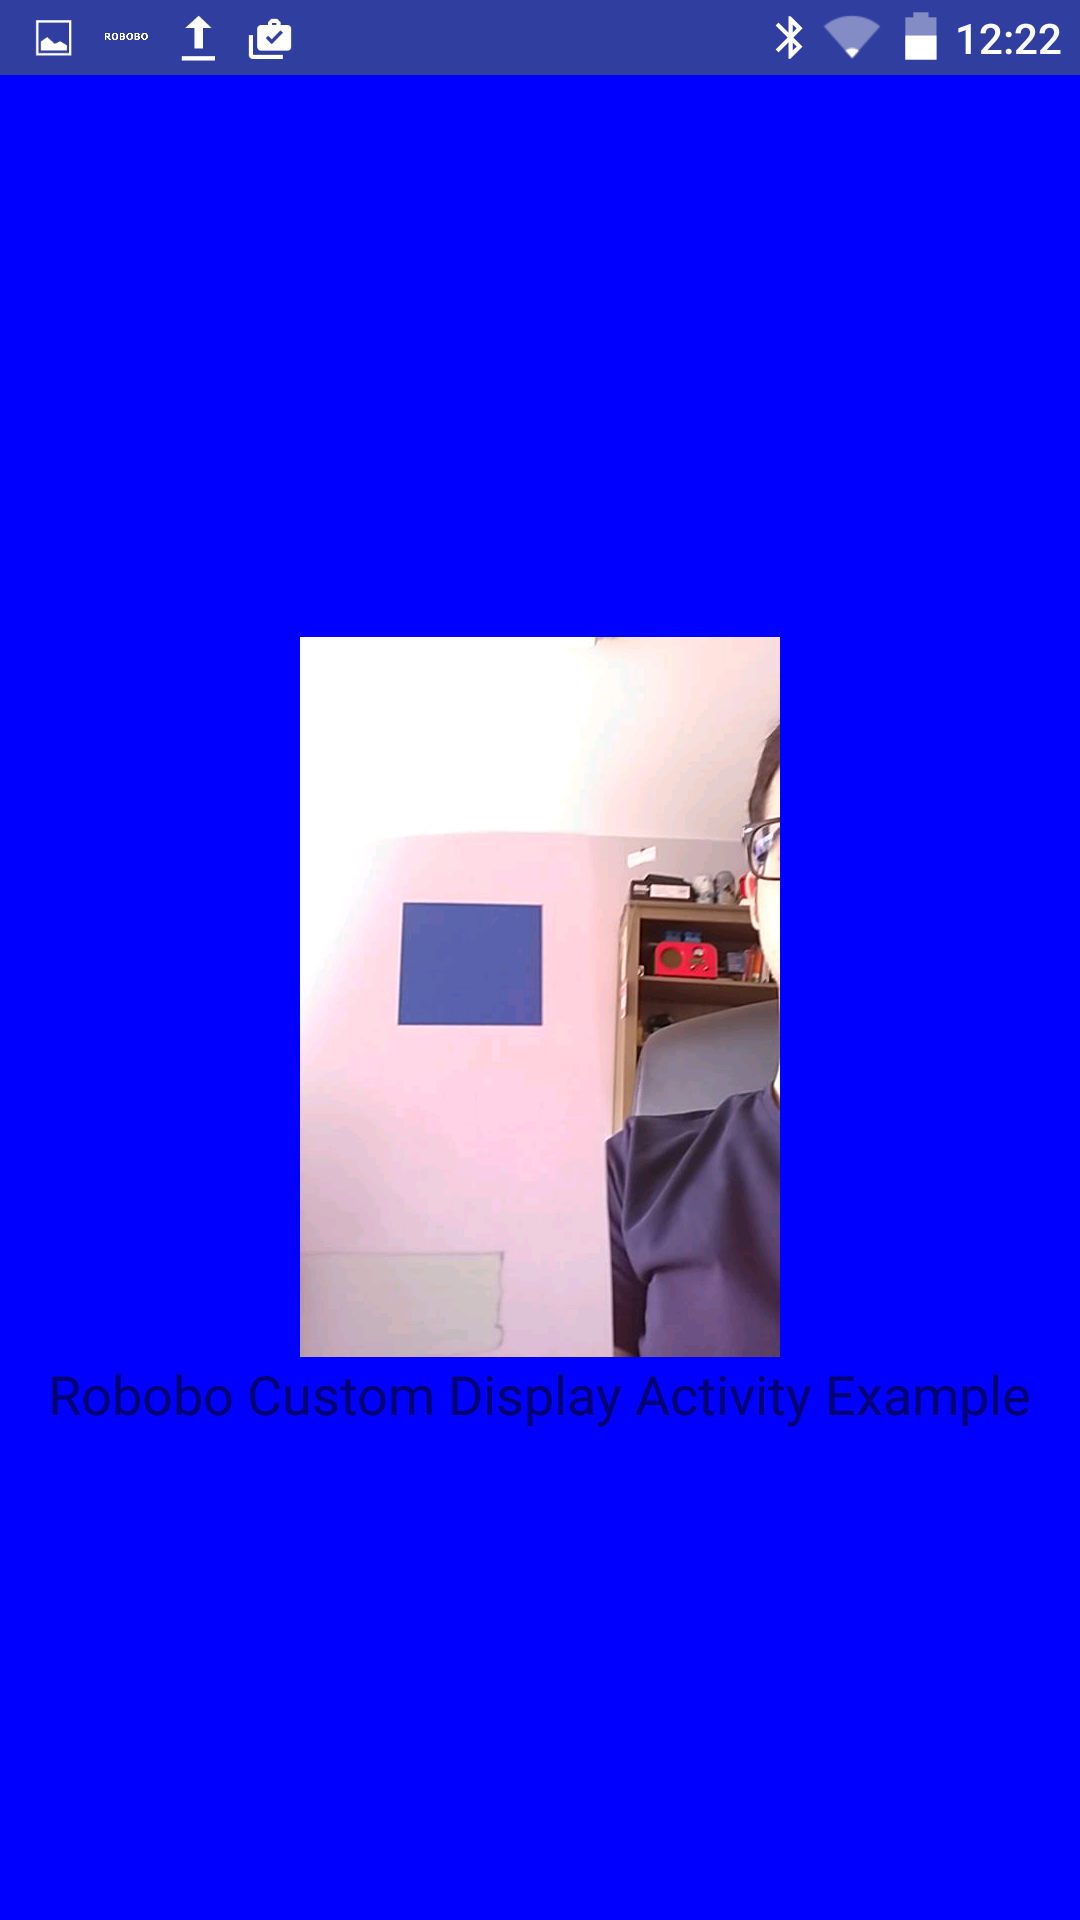
\includegraphics[width=1\linewidth]{imagenes/color_detection_blue.png}
\caption{Color azul detectado}
\label{fig:blue_color}

\end{minipage}\hfill
\begin{minipage}{0.45\textwidth}
\centering
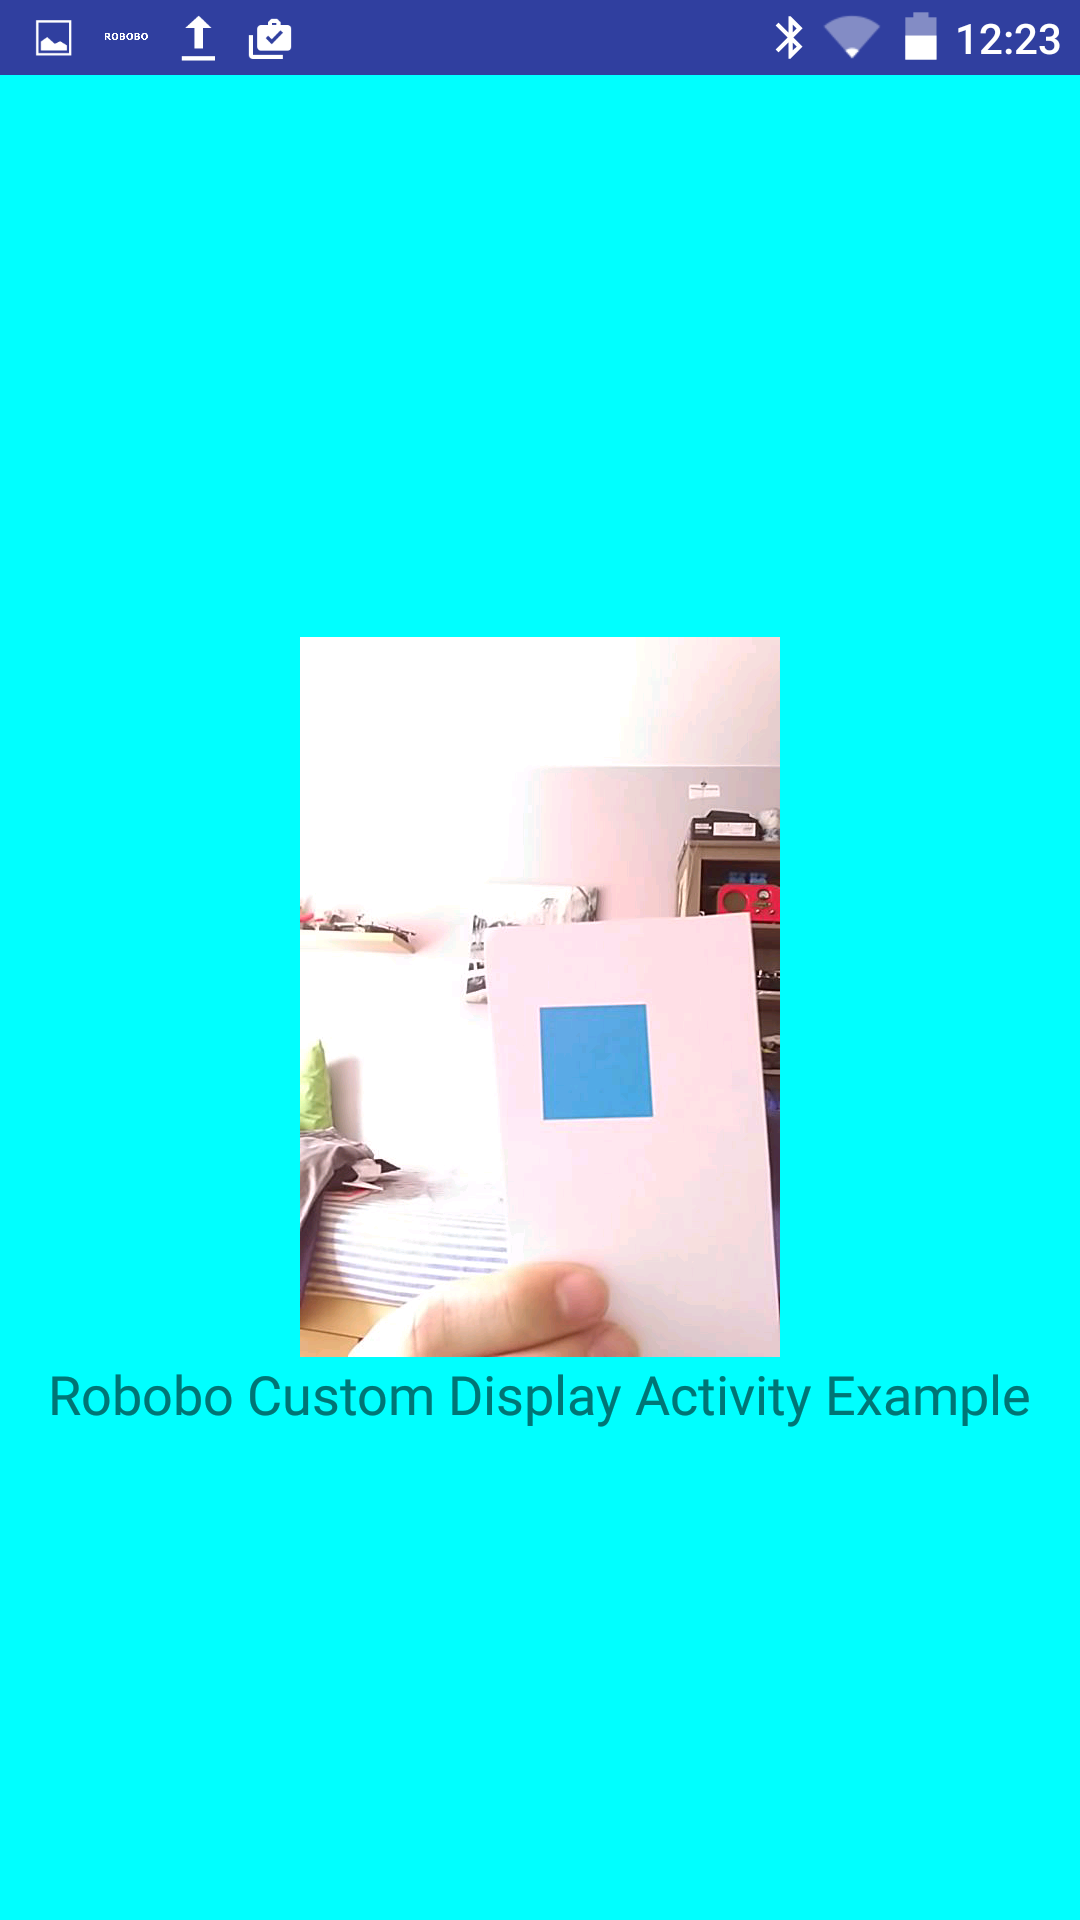
\includegraphics[width=1\linewidth]{imagenes/color_detection_cyan.png}

\caption{Color cían detectado}
\label{fig:cyan_color}

\end{minipage}
\end{figure}

\begin{figure}
\centering
\begin{minipage}{0.45\textwidth}
\centering
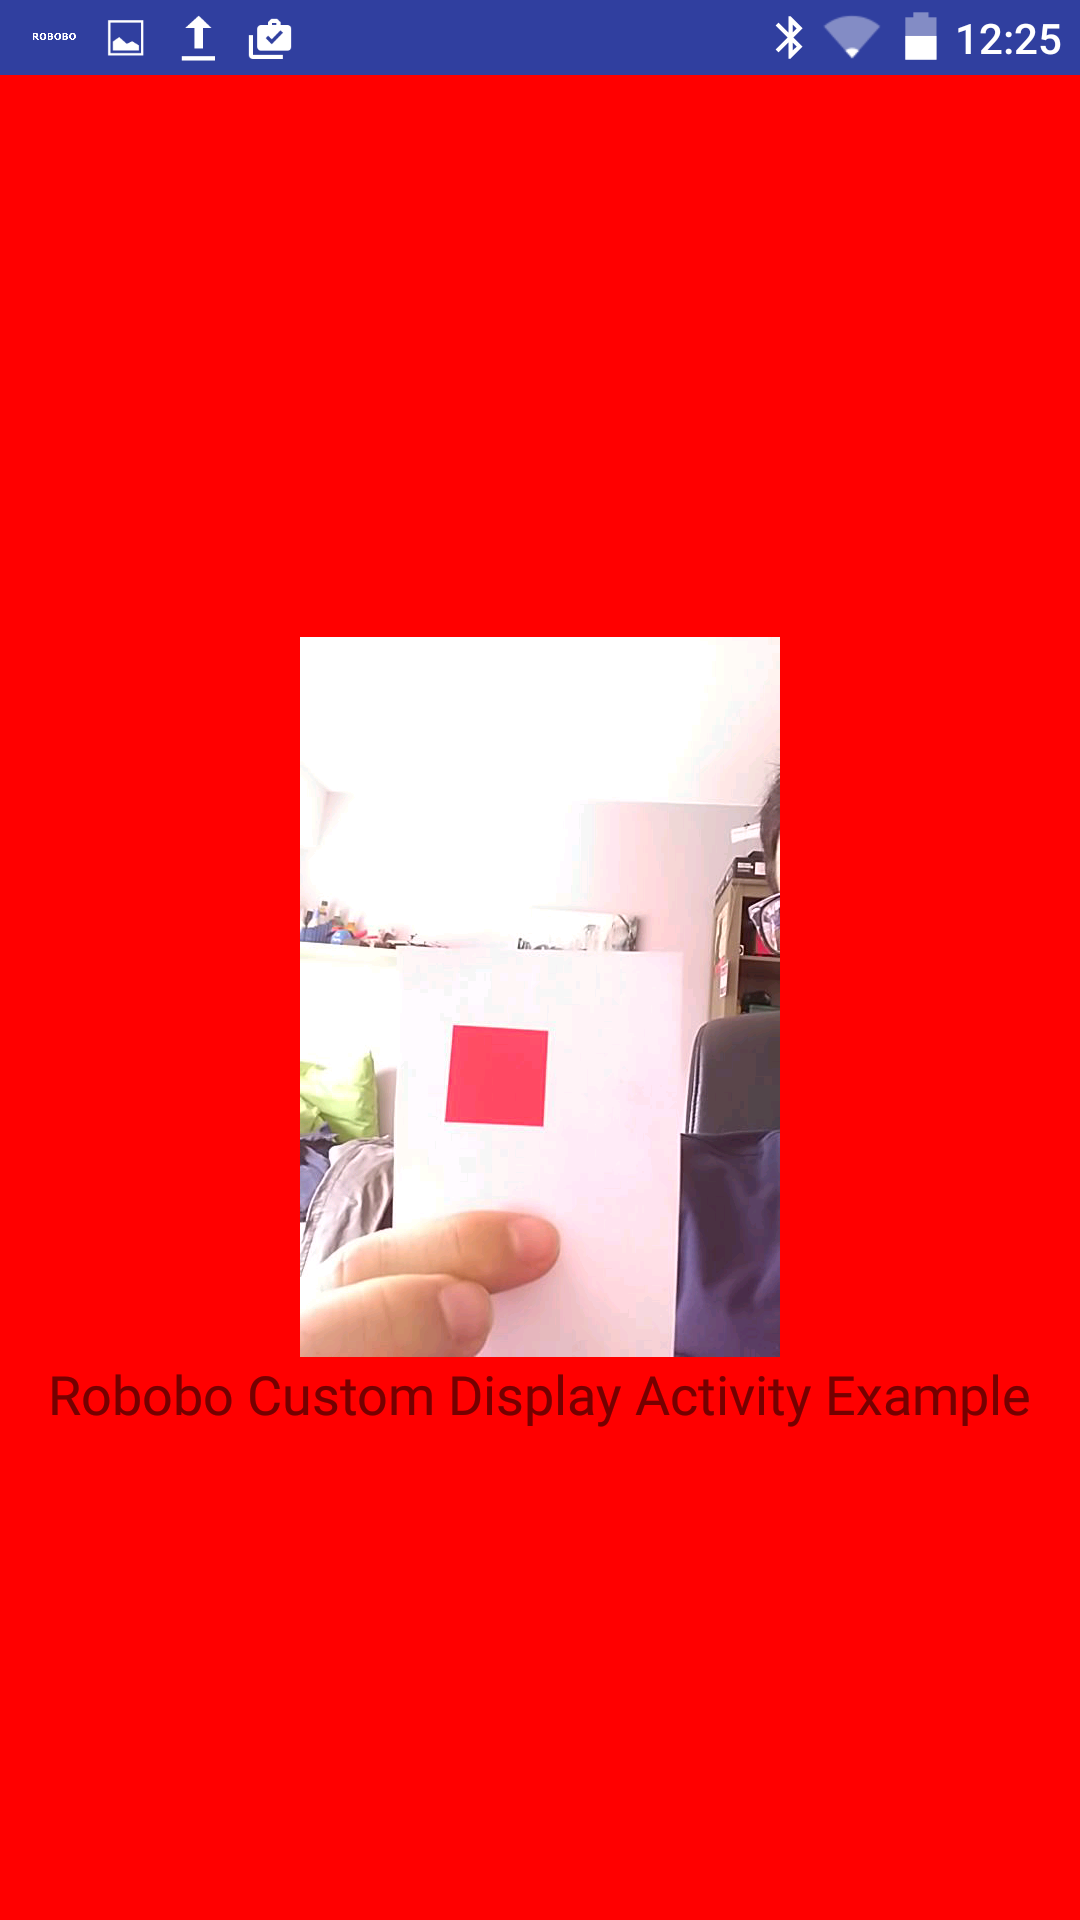
\includegraphics[width=1\linewidth]{imagenes/color_detection_red.png}
\caption{Color rojo detectado}
\label{fig:red_color}

\end{minipage}\hfill
\begin{minipage}{0.45\textwidth}
\centering
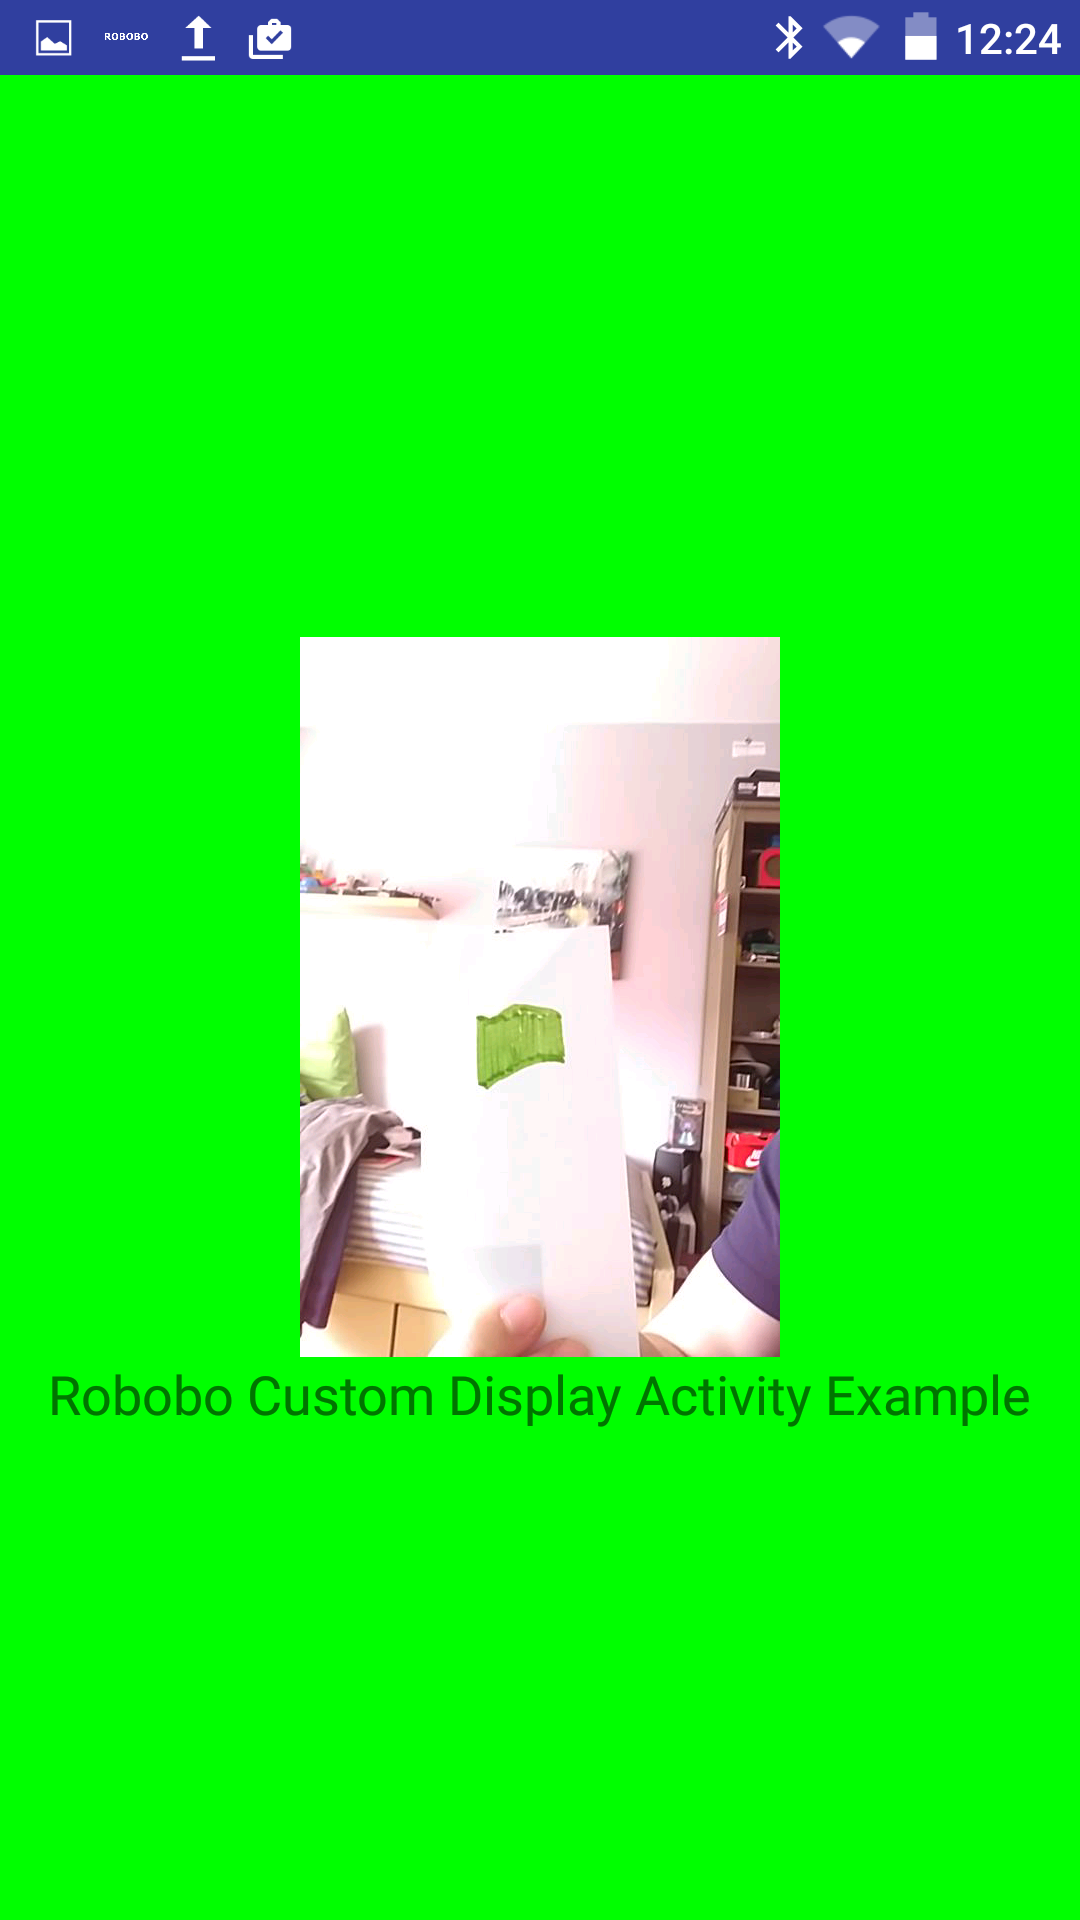
\includegraphics[width=1\linewidth]{imagenes/color_detection_green.png}

\caption{Color verde detectado}
\label{fig:green_color}

\end{minipage}
\end{figure}

\newpage
%%%%%%%%%%%%%%%%%%%%%%%%%%%%%%%%%%%%%%%%%%%%%%%%%%%%%%%%%%%%%%%%%%%%%%%%%%%%%%%%
\subsection{Paquete Messaging}
El subsistema Messaging aglomera las diferentes opciones de comunicación por mensajería de texto.

%%%%%%%%%%%%%%
\subsubsection{Módulo email}
\begin{figure}
	\centering
	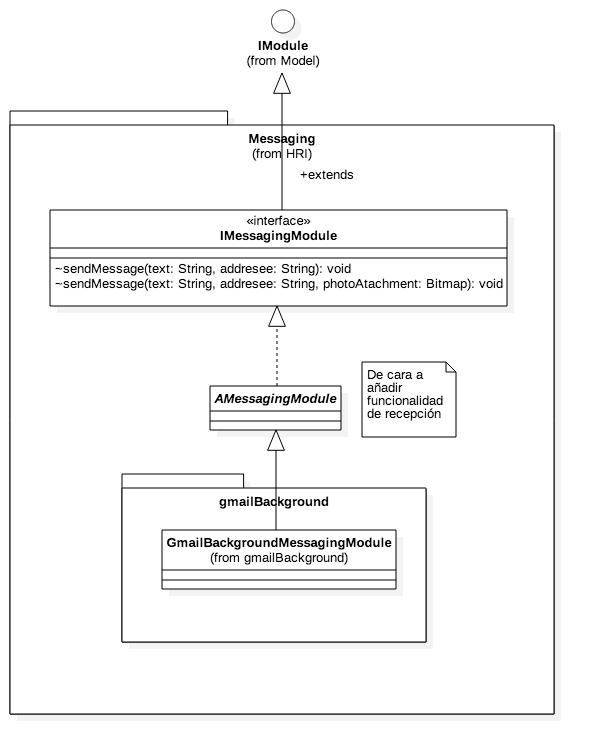
\includegraphics[width=0.7\linewidth]{imagenes/diagramas/MessagingModule.png}
	\caption{Módulo Email}
	\label{fig:email-module}
\end{figure}
El módulo Email(figura \ref{fig:email-module}) permite al usuario la comunicación mediante correo electrónico, pudiendo mandar tanto texto como imágenes, por ejemplo, las capturadas con el módulo \textit{BasicCamera}.

\paragraph*{GmailBackground\\}
Para implementar el módulo, se ha empleado la librería GmailBackGround \cite{gmailbg} la cual se presentó en la sección \ref{subsec:gmail-background} de este trabajo , que permite el envío de mensajes de correo electrónico con una cuenta de Gmail. El módulo se encuentra en la clase \textit{GmailBackgroundMessagingModule}.


\subsubsection*{Ejemplos de desarrollo}

Se aprovechó la aplicación de prueba comentada en la sección anterior para comprobar el correcto funcionamiento del módulo de mensajería.

\begin{figure}
	\centering
	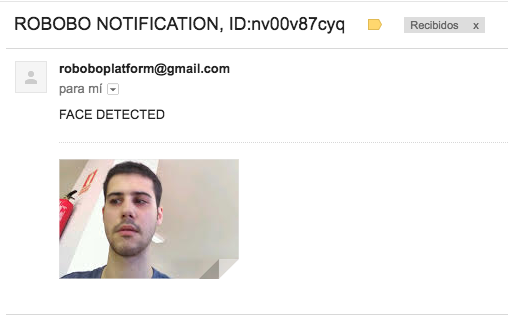
\includegraphics[width=1\linewidth]{imagenes/mail_example.png}
	\caption{Ejemplo de correo electrónico enviado}
	\label{fig:mail-example}
\end{figure}






